%!TEX root = ../master.tex
\chapter{Evaluation}\label{ch:evaluation}

This chapter will explain and describe the setup for the test, the procedure of the interview and results of the evaluation of the final prototype. 

\begin{figure}[!h] 
\centering
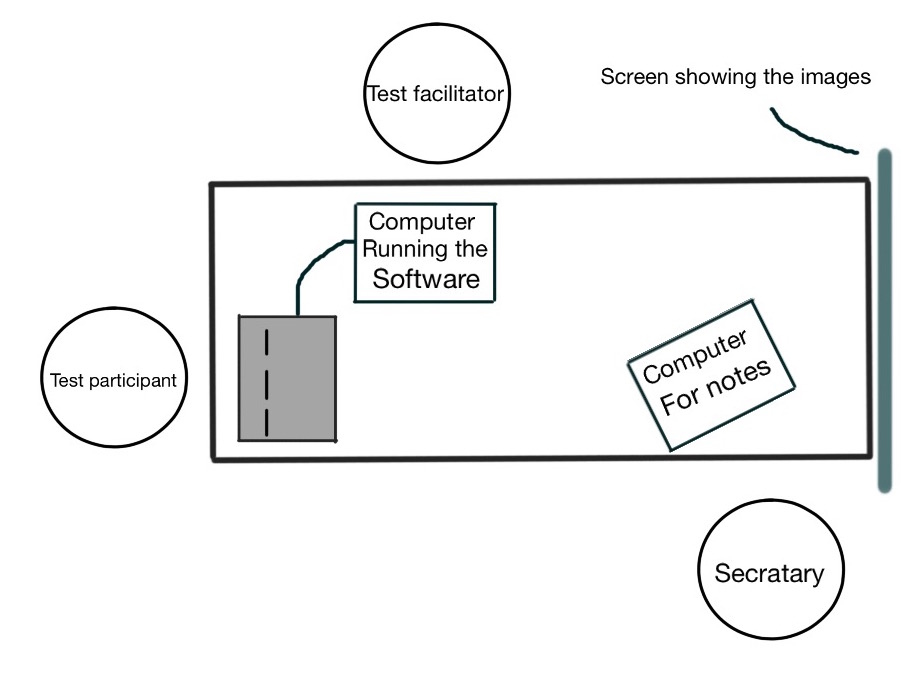
\includegraphics[width=0.7\textwidth]{testsetup}
\caption{\label{fig:testsetup} The test setup.}
\end{figure}

The final test was conducted on 15 test participants from Aalborg University through a semi-structured interview. The participants consisted of 14 students from Medialogy and one student from Art \& Technology. The test took place in a small secluded room located at Rendsburggade 14. It was conducted by a test facilitator who interviewed the participants and instructed them in the various tasks they had to do, while observing the software performed optimally. While the testing was being conducted, a secretary took notes of what the participants answered to the question as well as how they interacted with the product.
As seen on figure \ref{fig:testsetup}, the test participant was placed in front of the product with view to a TV screen that showed the image that is being audiolised. The two images that were audiolised was the 'Mona Lisa', as can be seen in Figure \ref{fig:monalisa}, and the a painting made by Asger Jorn called 'Trolden og Fuglene' as can be seen in Figure \ref{fig:asger}. The first image to be audiolised was the 'Mona Lisa' and the second one was 'Trolden of Fuglene'. Since the software and the image that was shown on the TV screen are independent of one another, the test facilitator had to change to the corresponding on the TV screen whenever a new image was audiolised. 

\begin{figure}[!h] 
\centering
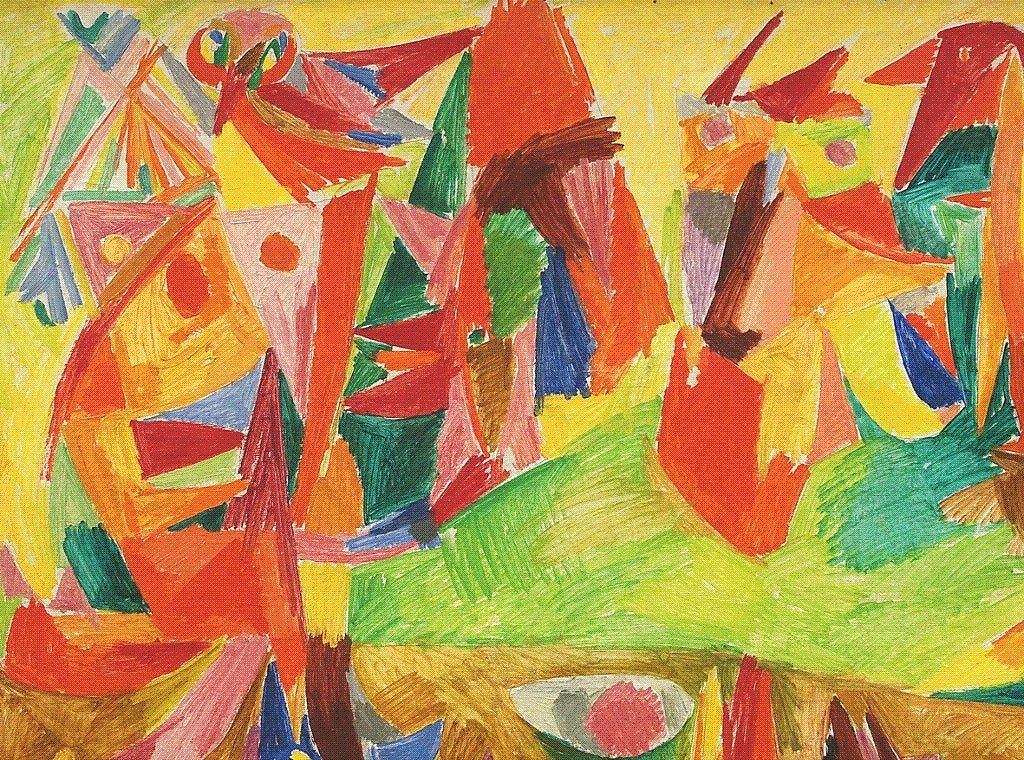
\includegraphics[width=0.5\textwidth]{asger}
\caption{\label{fig:asger} Asger Jorns 'Trolden og Fuglene' 1944.}
\end{figure}

\begin{figure}[!h] 
\centering
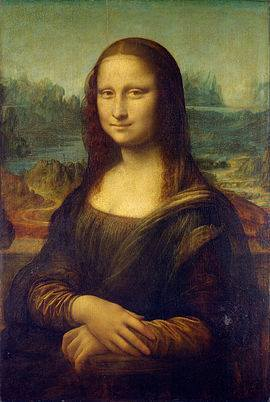
\includegraphics[width=0.5\textwidth]{monalisa}
\caption{\label{fig:monalisa} Leonardo Da Vinci 'Mona Lisa' 1503-1517.}
\end{figure}

The test was carried out by welcoming the test participant he/she was asked to sign a consent form. The test facilitator started the test by introducing the overall project and explaining what the participant was expected to do during the test such as thinking out loud (the full script can be seen in Appendix \ref{ch:appAinterviewscript}). The test participant was first asked what they immediately thought they had to do when they saw the interface. After the test participants gave their answer, the test facilitator turned on the audiolisation of 'Mona Lisa' and told the participant to play around with the sliders. The next questions was about the audio of the product; whether the participants could hear a difference between 'MIN' and 'MAX' as well as the difference between the individual filters. Before the audiolisation changed to 'Trolden og Fuglene', the participants were asked if the text on the interface helped them understand the product better. 
After changing to the audiolisation of 'Trolden og Fuglene' the participants were asked if they could hear a difference between the two images, and again, a difference between 'MIN' and 'MAX' and a difference between the individual filters. Lastly the participants were asked to give their final thoughts.

\section{Technical test of filters}
To make sure that the used filters work as intended, the frequency responses of the filters were plotted. By doing this, it is possible to see if the curve looks as it is supposed to, according to what filter is currently in use.

When testing the comb filter, the delay was adjusted to see if the frequency response changed appropriately. The two frequency response curves can be seen in Appendix \ref{ch:appBfrequencyresponse}. In both cases of short and long delay, the frequency response of the filter has a very distinct shape, with multiple sharp peaks and concave valleys in succession. This shape is very reminiscent of an upside-down comb, which is exactly what is desired of the frequency response of a comb filter.

When testing the bandpass filter, two phases of testing was conducted. Firstly, a static centre frequency was held, while the bandwidth of the filter was adjusted. Lastly, the bandwidth was held static, and the centre frequency was adjusted. The resulting four frequency response curves can be seen in Appendix \ref{ch:appBfrequencyresponse}. When looking at these curves, it is evident that when the bandwidth is low then many frequencies are rejected, while letting frequencies close to the centre frequency through. When the bandwidth is high, a large range of frequencies are let through, and only the frequencies furthest away from the centre frequency are rejected. The curve also moves in the desired direction, when increasing or decreasing the centre frequency.

When testing the high-shelf filter, three phases of testing was conducted. Firstly, the cut-off frequency was adjusted while the decibel gain and slope variable were held static. Then, the decibel gain was adjusted, while the cut-off frequency and slope variable were held static. Lastly, the slope variable was adjusted, while the cut-off frequency and decibel gain were held static. The resulting six frequency response curves can be seen in Appendix \ref{ch:appBfrequencyresponse}. The high plateau of the high-shelf filter decreases in width when increasing the cut-off frequency, which means that fewer of the higher frequencies are effected. When adjusting the decibel gain, the curve have a plateau when the decibel gain is positive, and becomes more of a valley when the decibel gain becomes negative. The slope between the middle line and the shelf becomes steeper as the slope variable is increased.

Therefore, all the filters do work as intended, as indicated by their frequency responses.

\section{Evaluation results and analysis}
The tables in this section (\ref{tab:comb}, \ref{tab:bandpass}, \ref{tab:highshelf}, \ref{tab:helptext}, \ref{tab:twoimagedifference}) shows the results from the evaluation. Table \ref{tab:comb}, \ref{tab:bandpass} and \ref{tab:highshelf} have both answers from each audiolisation when asking to hear the difference between 'MIN' and 'MAX'. This section contains the analysis of the test results. The analysis methods are outlined and then used. 

%Comb results
\begin{table}[!h]
\centering
\caption{}
\label{tab:comb}
\begin{tabular}{|l|c|c|c|c|c|c|c|c|c|c|c|c|c|c|c|c|c|}
\hline
\multicolumn{18}{|c|}{Can you hear the difference between the 'MIN' and 'MAX' on the Comb filter?} \\ \hline
\multicolumn{2}{|l|}{} & \multicolumn{15}{c|}{Amount of participants} & \textbf{Total} \\ \hline
\multirow{2}{*}{\begin{tabular}[c]{@{}l@{}}Mona \\ Lisa\end{tabular}} & Yes &  &  &  &  &  &  &  &  &  &  &  &  & X &  &  & \textbf{1} \\ \cline{2-18} 
 & No & X & X & X & X & X & X & X & X & X & X & X & X &  & X & X & \textbf{14} \\ \hline
\multirow{2}{*}{\begin{tabular}[c]{@{}l@{}}Asgar \\ Jorn\end{tabular}} & Yes &  &  &  &  &  &  &  &  &  &  & X &  & X &  &  & \textbf{2} \\ \cline{2-18} 
 & No & X & X & X & X & X & X & X & X & X & X &  & X &  & X & X & \textbf{13} \\ \hline
\end{tabular}
\end{table}

%Bandpass Results
\begin{table}[]
\centering
\caption{}
\label{tab:bandpass}
\begin{tabular}{|l|c|c|c|c|c|c|c|c|c|c|c|c|c|c|c|c|c|}
\hline
\multicolumn{18}{|c|}{Can you hear the difference between the 'MIN' and 'MAX' on the Bandpass filter?} \\ \hline
\multicolumn{2}{|l|}{} & \multicolumn{15}{c|}{Amount of participants} & \textbf{Total} \\ \hline
\multirow{2}{*}{\begin{tabular}[c]{@{}l@{}}Mona \\ Lisa\end{tabular}} & Yes & X & X &  & X & X & X & X &  & X & X & X & X & X &  &  & \textbf{11} \\ \cline{2-18} 
 & No &  &  & X &  &  &  &  & X &  &  &  &  &  & X & X & \textbf{4} \\ \hline
\multirow{2}{*}{\begin{tabular}[c]{@{}l@{}}Asgar \\ Jorn\end{tabular}} & Yes & X & X & X & X & X & X & X &  & X & X & X & X & X &  & X & \textbf{13} \\ \cline{2-18} 
 & No &  &  &  &  &  &  &  & X &  &  &  &  &  & X &  & \textbf{2} \\ \hline
\end{tabular}
\end{table}

%High shelf results
\begin{table}[]
\centering
\caption{}
\label{tab:highshelf}
\begin{tabular}{|l|c|c|c|c|c|c|c|c|c|c|c|c|c|c|c|c|c|}
\hline
\multicolumn{18}{|c|}{Can you hear the difference between the 'MIN' and 'MAX' on the High Shelf filter?} \\ \hline
\multicolumn{2}{|l|}{} & \multicolumn{15}{c|}{Amount of participants} & \textbf{Total} \\ \hline
\multirow{2}{*}{\begin{tabular}[c]{@{}l@{}}Mona \\ Lisa\end{tabular}} & Yes & X & X & X & X & X & X & X & X & X & X & X & X & X & X & X & \textbf{15} \\ \cline{2-18} 
 & No &  &  &  &  &  &  &  &  &  &  &  &  &  &  &  & \textbf{0} \\ \hline
\multirow{2}{*}{\begin{tabular}[c]{@{}l@{}}Asgar \\ Jorn\end{tabular}} & Yes & X & X & X & X & X & X & X & X & X & X & X & X & X & X & X & \textbf{15} \\ \cline{2-18} 
 & No &  &  &  &  &  &  &  &  &  &  &  &  &  &  &  & \textbf{0} \\ \hline
\end{tabular}
\end{table}

%Is the "help text" useful you you?
\begin{table}[!h]
\centering
\caption{}
\label{tab:helptext}
\begin{tabular}{|l|c|c|c|c|c|c|c|c|c|c|c|c|c|c|c|c|}
\hline
\multicolumn{17}{|c|}{Is the "help text" usefull to you?} \\ \hline
 & \multicolumn{15}{c|}{Amount of participants} & \textbf{Total} \\ \hline
Yes &  & X & X & X & X & X & X & X & X & X & X & X & X & X & X & \textbf{14} \\ \hline
No & X &  &  &  &  &  &  &  &  &  &  &  &  &  &  & \textbf{1} \\ \hline
\end{tabular}
\end{table}

%Can you hear a difference between the two images?
\begin{table}[!h]
\centering
\caption{}
\label{tab:twoimagedifference}
\begin{tabular}{|l|c|c|c|c|c|c|c|c|c|c|c|c|c|c|c|c|}
\hline
\multicolumn{17}{|c|}{Can you hear a difference between the two images?} \\ \hline
 & \multicolumn{15}{c|}{Amount of participants} & \textbf{Total} \\ \hline
Yes & X & X & X & X & X & X & X & X & X & X & X & X & X & X & X & \textbf{15} \\ \hline
No &  &  &  &  &  &  &  &  &  &  &  &  &  &  &  & \textbf{0} \\ \hline
\end{tabular}
\end{table}

For statistical analysis of quantitative data, Fisher's exact test is used to determine whether there is a connection between explanatory variables and their contingencies. This test is specifically concerned with the influence the two different images have on our results. Binomial tests are used to determine the significance of our results. An significance value $\alpha$ of 0.05 is used.

The product must be able to audiolise the image. For this criteria to be fulfilled, individual images must produce audio that is distinct. The user test shows that images produce a unique sound. This can be seen in the fact that all test participants could hear a clear difference between the colourful Asger Jorn painting and the darker Mona Lisa painting ($p=6.104e-5$). 

The effects that are applied to this audiolisation must be alterable by the user. The technical test shows that the audio filters are applied as desired - the filter responses match what is expected from the respective types of filter. There is an underlying assumption to this criteria that this effect must be discernable by the user, otherwise there is no point to it. Using Fisher's exact test it is first determined whether the image has an influence on whether the user can hear the effect. There is no significant correlation between the image used and the users ability to hear the affect for any of the filters ($p_{comb}=1$, $p_{bandpass}=0.6513$, $p_{highshelf}=1$). Then we determine whether users can hear a difference between a filter being a applied or not applied. Users determined that they could hear the bandpass filter ($p=0.001431$) and the high shelf filter ($p=1.863e-09$). They also determined they could NOT hear the comb filter ($p=8.43e-06$).

Finally the product must be usable. The interface was clear for all the participants and they knew how to use it, either by looking at the help text or at the sliders. None of the test participants had any trouble manipulating with the sliders. Nine of the participants did not know the terms of the different filters, but they could distinguish a change in the output when manipulating with the sliders. However, all users found the help text helpful. This indicates that the principle of using text labels to explain certain elements of this kind of interface is sound, but that the current implementation of this is problematic. The biggest issue here is probably that the labels make use of technical language which only provides useful information for expert users.
 
